\pagenumbering{arabic}

\section{Booting a PC}

\subsection{Computer Boot }


\subsubsection{Simulating The X86}
In this experiment, we chose QEMU to simulate a real computer. The use of QEMU is as follows.
\begin{figure}[htbp]
\centering
\begin{minipage}[t]{0.48\textwidth}
\centering
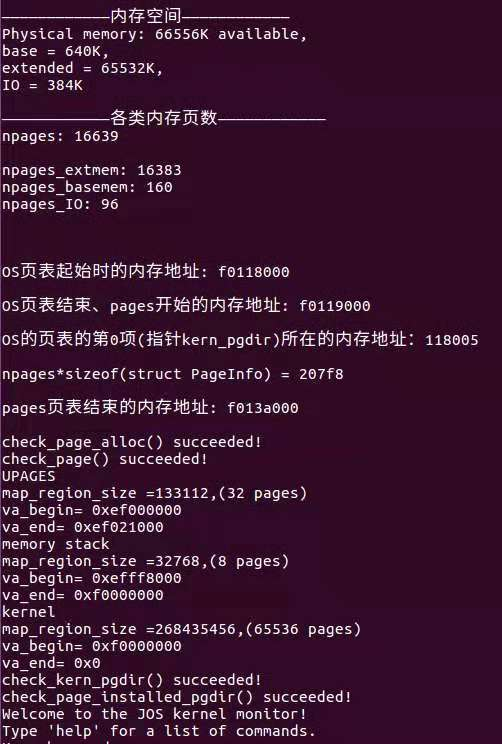
\includegraphics[width=6cm]{figure/make_qemu}
\caption{make qemu}
\end{minipage}
\begin{minipage}[t]{0.48\textwidth}
\centering
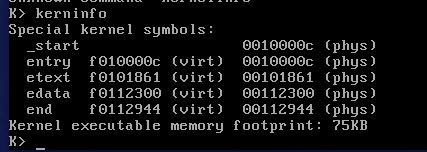
\includegraphics[width=6cm]{figure/kerninfo}
\caption{kerninfo}
\end{minipage}
\end{figure}

Through the above two instructions, we can see that the kernel information has been output in the console. It can be seen that QEMU can function as a simulation computer and the system can run normally.
\subsubsection{The PC's Physical Address Space}
The approximate physical distribution of the physical memory of the pc is as follows
\begin{figure}[H]
  \centering
  % Requires \usepackage{graphicx}
  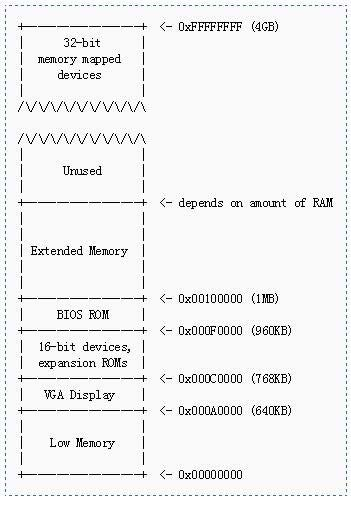
\includegraphics[width=0.8\linewidth]{figure/physical_address}\\
  \caption{i文件部分代码}\label{2}
\end{figure}
The 384KB of physical address range 0x000A0000~0x000FFFFF is reserved for hardware devices such as VGA display buffers. The most important part of this part is as the basic input and output system (BIOS, Basic)Input/Output System) The 64KB area of ​​0x000F0000~0x000FFFFF. The BIOS handles the basic initialization tasks of the system, such as activating the display, checking memory, and so on. After completing these initialization tasks, the BIOS loads the operating system from a floppy disk, hard drive, optical drive, or network and transfers control to the operating system.

On the modern PC, the 0x000A0000~0x00100000 segment is left as a "hole", which divides the memory into two segments. The lower 640K is called "low-segment memory", and the remaining high-address portion is expanded memory. At the same time, in the highest part of the physical address space, above all physical RAM, some are also reserved by the BIOS for 32-bit PCI devices.
\subsubsection{BIOS}
\begin{figure}[H]
  \centering
  % Requires \usepackage{graphicx}
  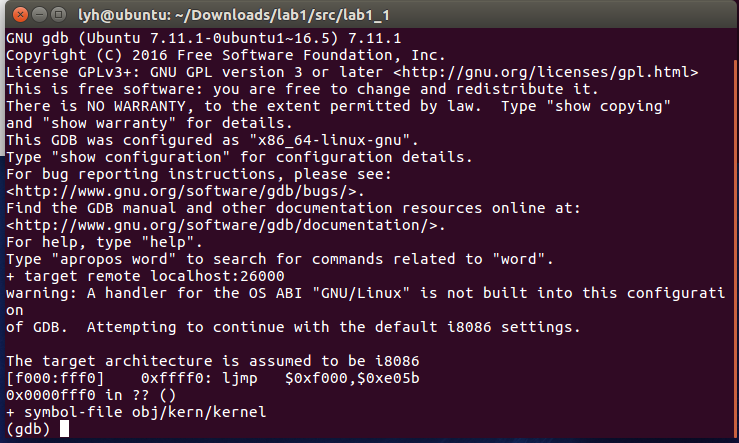
\includegraphics[width=0.8\linewidth]{figure/gdb}\\
  \caption{gdb}\label{2}
\end{figure}

In the running content of gdb, we can see the first instruction that gdb runs (as shown below). In this instruction, we can see that pc starts from CS = 0xf000 and IP = 0xfff0. The execution of the first sentence is a JMP operation that jumps to CS = 0xf000 and IP = 0xe05b. Since the modern CPU is divided into real mode and protection mode, it runs in real mode at startup and runs in protected mode after startup. The BIOS is the software that runs when the PC first starts up, so it must work in real mode. So the real address of the jump is 0xf000<<4+0xe05b = 0xfe05b.



\begin{figure}[H]
  \centering
  % Requires \usepackage{graphicx}
  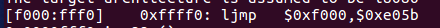
\includegraphics[width=0.8\linewidth]{figure/first_commond}\\
  \caption{The first instruction of the BIOS}\label{2}
\end{figure}


\subsection{Boot Loader}
For PCs, floppy disks and hard disks can be divided into 512-byte areas called sectors. A sector is the smallest granularity of a disk operation. Each read or write operation must be one or more sectors. If a disk can be used to boot the operating system, the first sector of the disk is called the boot sector. The boot loader program described in this section is located in this boot sector. When the BIOS finds a floppy disk or hard disk that can be booted, it loads the 512-byte boot sector into the memory address 0x7c00~0x7dff.
The boot loader must perform two main functions.

 1. First, the boot loader will convert the processor from real mode to 32-bit protected mode, because only in this mode the software can access more than 1MB of content.

 2. The boot loader can then access the IDE disk device registers directly from the disk by using x86 specific IO instructions.

For the boot loader, there is a file that is important, obj/boot/boot.asm. This file is a disassembled version of our real-run boot loader program. So we can compare it with its source code, boot.S and main.c.

\subsubsection{Question \Rmnum{1}}
Set a breakpoint at address 0x7c00, which is where the boot sector will be loaded. Continue execution until that breakpoint. Trace through the code in boot/boot.S, using the source code and the disassembly file obj/boot/boot.asm to keep track of where you are. Also use the x/i command in GDB to disassemble sequences of instructions in the boot loader, and compare the original boot loader source code with both the disassembly in obj/boot/boot.asm and GDB.

Trace into bootmain() in boot/main.c, and then into readsect(). Identify the exact assembly instructions that correspond to each of the statements in readsect(). Trace through the rest of readsect() and back out into bootmain(), and identify the begin and end of the for loop that reads the remaining sectors of the kernel from the disk. Find out what code will run when the loop is finished, set a breakpoint there, and continue to that breakpoint. Then step through the remainder of the boot loader.
\begin{flushleft}
1) At what point does the processor start executing 32-bit code? What exactly causes the switch from 16- to 32-bit mode?\\
2) What is the last instruction of the boot loader executed, and what is the first instruction of the kernel it just loaded?\\
3) Where is the first instruction of the kernel?\\
4) How does the boot loader decide how many sectors it must read in order to fetch the entire kernel from disk? Where does it find this
information?\\
\end{flushleft}

The BIOS will copy the boot sector to the address 0x7c00, so the starting address of boot.S is 0x7c00.So we enter b *0x7c00 in the gdb window, then enter c, which means continue to run to the breakpoint, where we enter x/30i 0x7c00.This gdb instruction disassembles the instructions stored in 0x7c00 and the next 30 bytes of memory.
\begin{figure}[H]
  \centering
  % Requires \usepackage{graphicx}
  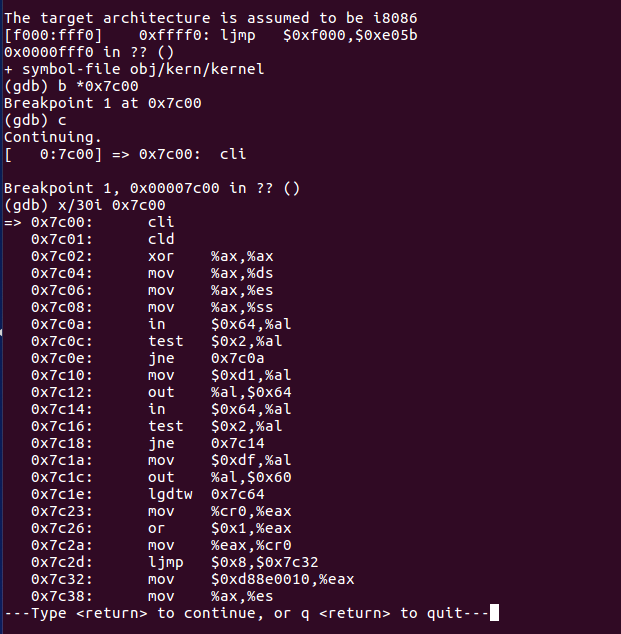
\includegraphics[width=0.8\linewidth]{figure/set_breakpoint}\\
  \caption{Disassembly}\label{2}
\end{figure}

We take it directly with boot.S and at obj/boot/boot.asm

\begin{figure}[H]
\centering
\begin{minipage}[t]{0.7\textwidth}
\centering
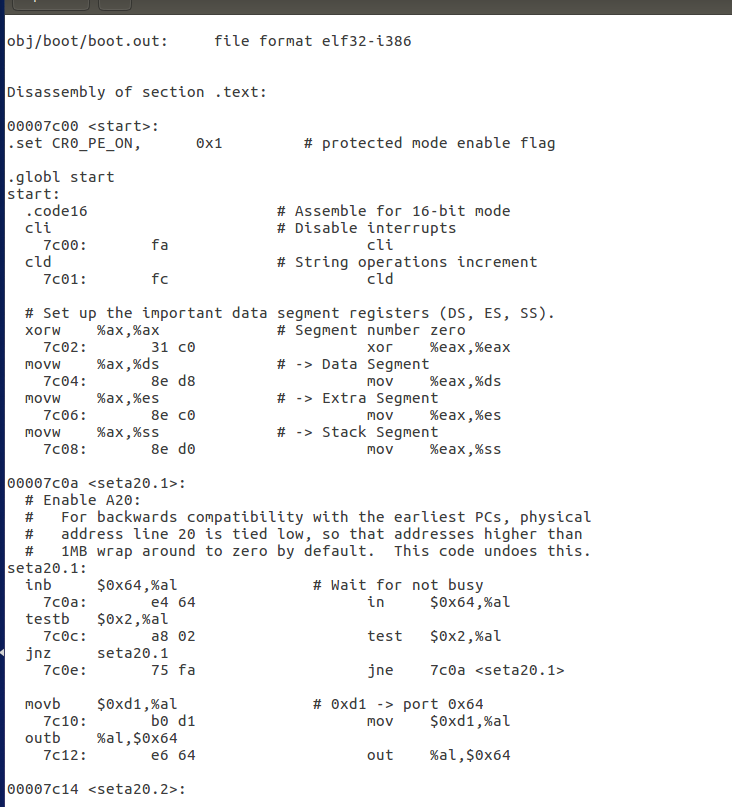
\includegraphics[width=10cm]{figure/boot_asm}
\caption{boot.asm}
\end{minipage}
\begin{minipage}[t]{0.7\textwidth}
\centering
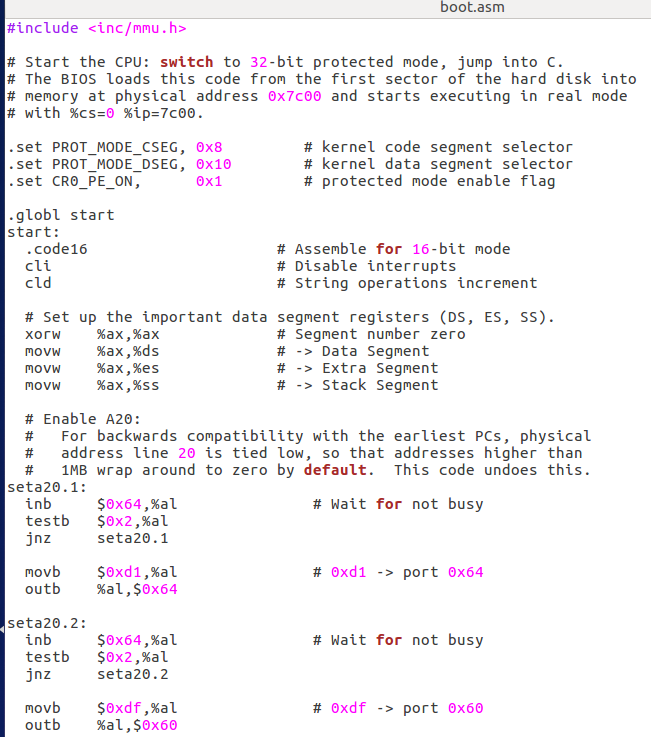
\includegraphics[width=10cm]{figure/boot_s}
\caption{boot.s}
\end{minipage}
\end{figure}

By comparing we can find that the three are not different in the instruction, but in the source code, we specify a lot of identifiers such as set20.1. Initially, these identifiers are converted to real physical addresses after being assembled into machine code. For example, set20.1 is converted to 0x7c0a, then this correspondence is listed in OBJ's /boot/boot.asm, but in the real case, in the first case, you can't see set20. 1 identifier, completely real physical address.


Then according to the title indication, we first traced to the bootmain function, we found that bootmain is at address 0x7c45, so we set the breakpoint there, and run here, then set the breakpoint at the readsect (0x7c7c) and jump here After using the si command to step through, found that into the waitdisk function (ox7c6a)
\begin{figure}[H]
  \centering
  % Requires \usepackage{graphicx}
  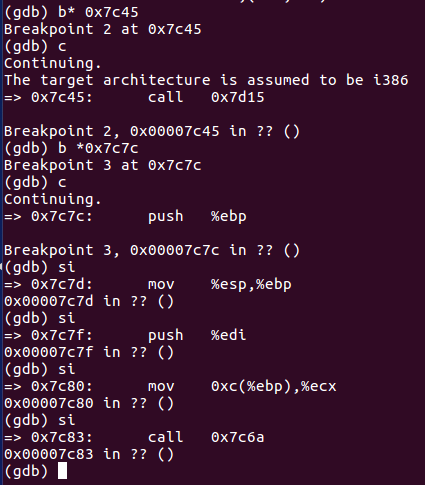
\includegraphics[width=0.8\linewidth]{figure/to_wait_disk}\\
  \caption{call bootmain}\label{2}
\end{figure}
In boot.asm we can find the corresponding content of 0x7d6b. Jumping to here means ((void (*)(void)) (ELFHDR->e\_entry))() the function is executed, where the meaning of the e\_entry field of the ELF header is the first instruction of the executable. Virtual address. So the meaning of this sentence is to transfer control to the operating system kernel.
Then we find the end of the for statement in the file and jump to this location (0x7d6b).
\begin{figure}[H]
  \centering
  % Requires \usepackage{graphicx}
  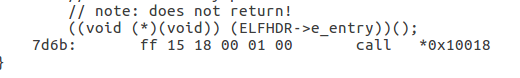
\includegraphics[width=0.8\linewidth]{figure/end_for}\\
  \caption{end loop}\label{2}
\end{figure}
\begin{figure}[H]
  \centering
  % Requires \usepackage{graphicx}
  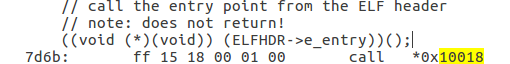
\includegraphics[width=0.8\linewidth]{figure/7d6b}\\
  \caption{the instruction after loop}\label{2}
\end{figure}
\vspace{9pt}
\begin{flushleft}
{\Large Answer:}\\
1)\\
\qquad As we discussed earlier, When the PC starts up, the CPU runs in real mode (real mode), and when it enters the operating system kernel, it will run in protected mode (protected mode). When entering protection mode, the CPU will switch from 16 bits to 32 bits.
\begin{figure}[H]
  \centering
  % Requires \usepackage{graphicx}
  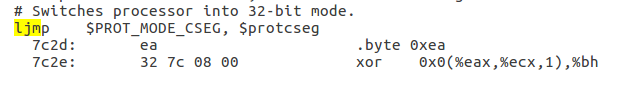
\includegraphics[width=0.8\linewidth]{figure/mode_change}\\
  \caption{mode change}\label{2}
\end{figure}
\qquad In the boot.S file, the computer first works in real mode, this time is the 16bit working mode. As can be seen from the above figure, when the "ljmp \$PROT\_MODE\_CSEG, \$protcseg" statement is run, the 32-bit working mode is officially entered. The root cause is that the CPU is working in protected mode at this time.\\
2)\\
\begin{figure}[H]
  \centering
  % Requires \usepackage{graphicx}
  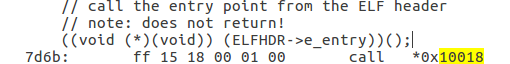
\includegraphics[width=0.8\linewidth]{figure/7d6b}\\
  \caption{the instruction after loop}\label{2}
\end{figure}
\qquad As shown in the figure above, the last statement executed by the boot loader is the last statement in the bootmain subroutine "((void (*)(void)) (ELFHDR->e\_entry))(); ", that is, jump to the operating system The starting instruction of the kernel program.
This first instruction is located in the /kern/entry.S file, the first sentence movw \$0x1234, 0x472\\
3)\\
\qquad The first instruction is in the /kern/entry.S file.\\
4)\\
\qquad First, how many segments are shared by the operating system, and how many sectors are in each segment are located in the Program Header Table in the operating system file. Each entry in this table corresponds to a segment of the operating system. And the content of each entry includes the size of the segment, the segment start address offset, and the like. So if we can find this table, we can determine how many sectors the kernel occupies by the information provided by the table entry.
Then the information about where this table is stored is stored in the ELF header information of the operating system kernel image file.\\
\end{flushleft}

\subsubsection{Loading kernel}
An executable ELF file consists of three main parts: a file header with loading information, followed by a program segment table, followed by several program segments. Each of these segments is a piece of continuous code or data. They are first loaded into memory when they are run. The job of the boot loader is to load them into memory.We can use the following instructions to examine the names, sizes, and addresses of all segments in the JOS kernel.

{\color{red} objdump -h obj/kern/kernel}

\begin{figure}[H]
  \centering
  % Requires \usepackage{graphicx}
  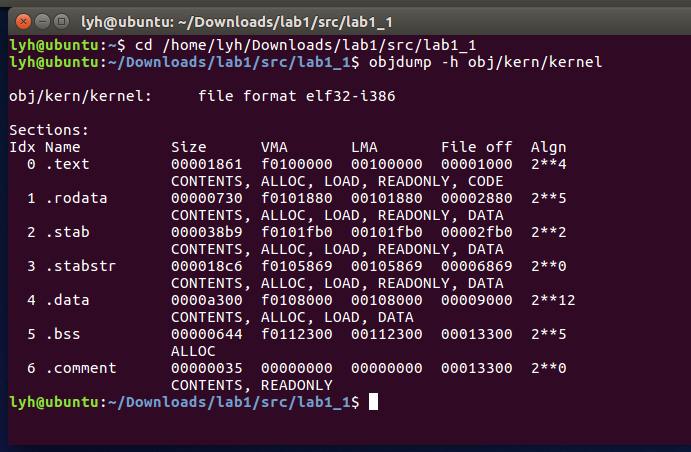
\includegraphics[width=0.8\linewidth]{figure/kernel_sections}
  \caption{All segment information in the kernel}\label{2}
\end{figure}

\subsubsection{Connection address and load address}
There are two more important fields in each segment, VMA (link address), LMA (load address). The load address represents the physical address of the segment after it is loaded into memory. The link address refers to the logical address to which this segment is expected to be stored.

Each ELF file has a Program Headers Table that indicates which parts of the ELF file are loaded into memory and the addresses that are loaded into memory. We get the information of the Program Headers Table of the kernel by entering the following instructions:

{\color{red} objdump -x obj/kern/kernel}
\begin{figure}[H]
  \centering
  % Requires \usepackage{graphicx}
  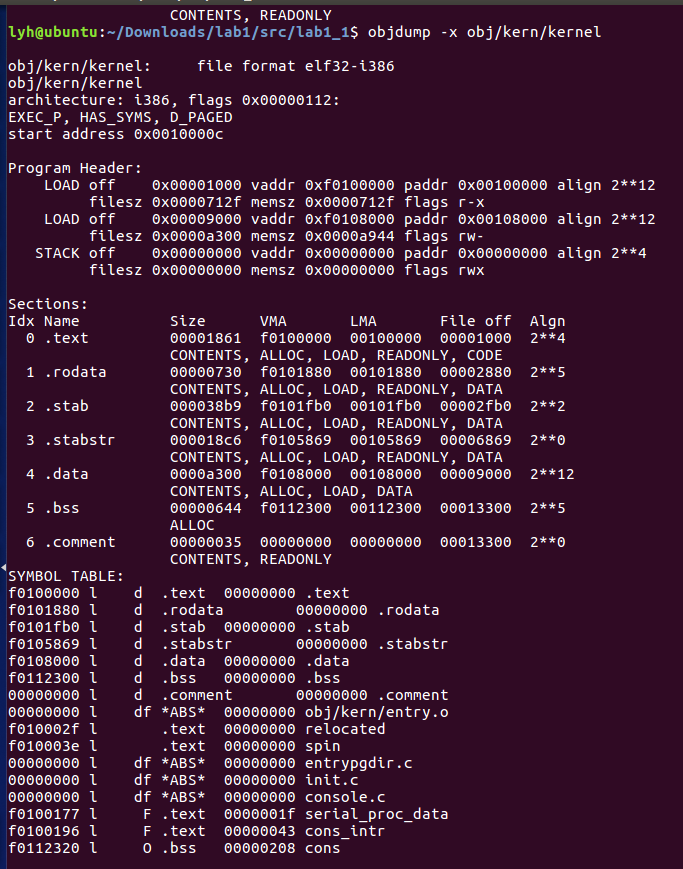
\includegraphics[width=0.8\linewidth]{figure/kernel_table}
  \caption{Kernel's Program Headers Table information}\label{2}
\end{figure}

\subsection{The Kernel}
\subsubsection{Question}
\begin{figure}[H]
  \centering
  % Requires \usepackage{graphicx}
  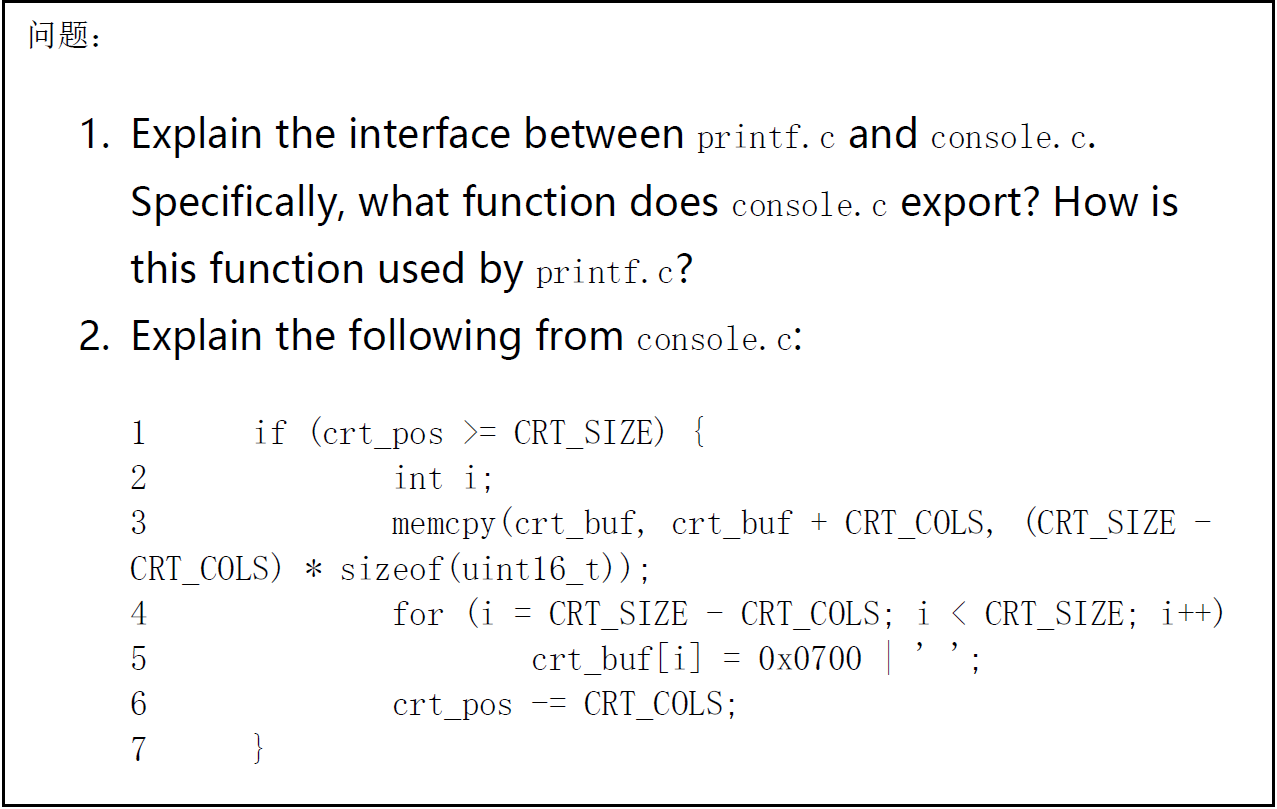
\includegraphics[width=0.8\linewidth]{figure/question}
\end{figure}
{\Large Answer:}\\
\begin{flushleft}
1)\\
\qquad Console.c defines how to display a character to the console, which is on top of our display, which includes many operations on the IO port.What is defined in printf.c is the top-level formatted output subroutine we will use in programming, such as printf, sprintf, and so on. The function exported by console.c which is used by printf.c is cputchar(),
That function prints a character in the parellel port and in the display.

\qquad Specific call relationship: cprintf -> vcprintf -> putch -> cputchar. Kernel's cprintf() function calls vprintfmt() (from lib/printfmt.c) to
Actually print in the console, vprintfmt() does the needed formatting and
Then call a function passed to it to actually print in the display.
\end{flushleft}
\begin{figure}[H]
  \centering
  % Requires \usepackage{graphicx}
  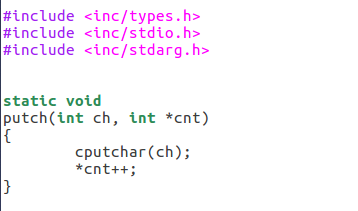
\includegraphics[width=0.8\linewidth]{figure/interface}
  \caption{Function call}\label{2}
\end{figure}
\begin{flushleft}
2)\\
\qquad Crt\_buf: This is a character array buffer that holds the characters to be displayed on the screen.\\

\qquad Crt\_pos: This indicates the position of the current last character displayed on the screen.\\
\qquad When crt\_pos >= CRT\_SIZE, where CRT\_SIZE = 80*25, since we know that the value range of crt\_pos is 0~(80*25-1), if this condition is true, it means that the content output on the screen has exceeded one page. . So at this point you have to scroll the page up one line, that is, put the original line 1~79 on the current 0~78 line, and then replace the line 79 with a line of spaces (of course not all spaces, 0 characters) To display the character int c) you entered. So the memcpy operation is to copy the contents of lines 1~79 in the crt\_buf character array to the position of lines 0~78. The next for loop is to turn the last line, line 79 into a space. Finally, you need to modify the value of crt\_pos.
\end{flushleft}

\subsubsection{Use virtual memory}
As we discussed earlier, the computer is divided into real mode and protected mode when it starts up.When running the boot loader, the link address (virtual address) and the load address (physical address) in the boot loader are the same. But when you enter the kernel, the two addresses are no longer the same.
In the virtual address space, we put the operating system at the high address 0xf0100000, but in the actual memory we store the operating system in a low physical address space, such as 0x00100000. Then when the user program wants to access an instruction of an operating system kernel, the first is to give a high virtual address, and then the virtual address is mapped to a real physical address by a certain mechanism in the computer, thus solving the above problem. . Then such an organization is usually implemented through segment management and paging management.
\subsubsection{Homework \Rmnum{1}}
{\Large We have omitted a small fragment of code - the code necessary to print octal numbers using patterns of the form "\%o". Find and fill in this code fragment.}

\begin{flushleft}
{\Large Answer}\\
\qquad To answer this question, we should first understand the three files $\backslash$ kern $\backslash$  printf.c, $\backslash$ kern $\backslash $ console.c, $\backslash$ lib $\backslash$ printfmt.c to understand the relationship between them.
\qquad First of all, we should pay attention to the console.c file, the most important of which is the cputchar subroutine. We can find that this program is the IO control program of the high-level console. In addition, the implementation of cputchar is actually done by calling cons\_putc. And the function of the cons\_putc program is to output a character to the console.
\end{flushleft}
\begin{figure}[H]
  \centering
  % Requires \usepackage{graphicx}
  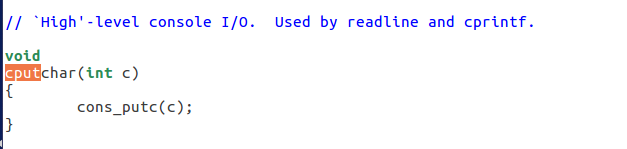
\includegraphics[width=0.8\linewidth]{figure/cputchar}
  \caption{cputchar}\label{2}
\end{figure}
\begin{figure}[H]
  \centering
  % Requires \usepackage{graphicx}
  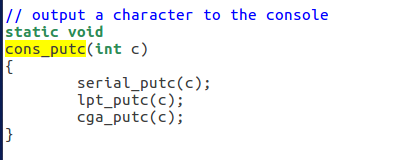
\includegraphics[width=0.8\linewidth]{figure/cons_putc}
  \caption{cons\_putc}\label{2}
\end{figure}
\qquad Then, let's focus on the printfmt.c file. By commenting, we can see that the subroutine defined in this file is the key to the information we can use to directly output information to the screen during programming using the printf function.
\begin{figure}[H]
  \centering
  % Requires \usepackage{graphicx}
  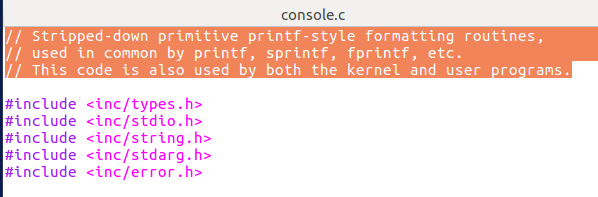
\includegraphics[width=0.8\linewidth]{figure/printfmt}
  \caption{printfmt}\label{2}
\end{figure}
Finally, let's take a look at the printf.c file.By commenting, we can see that the function of this file is to implement the simple implementation of cprintf console output for the kernel.
\begin{figure}[H]
  \centering
  % Requires \usepackage{graphicx}
  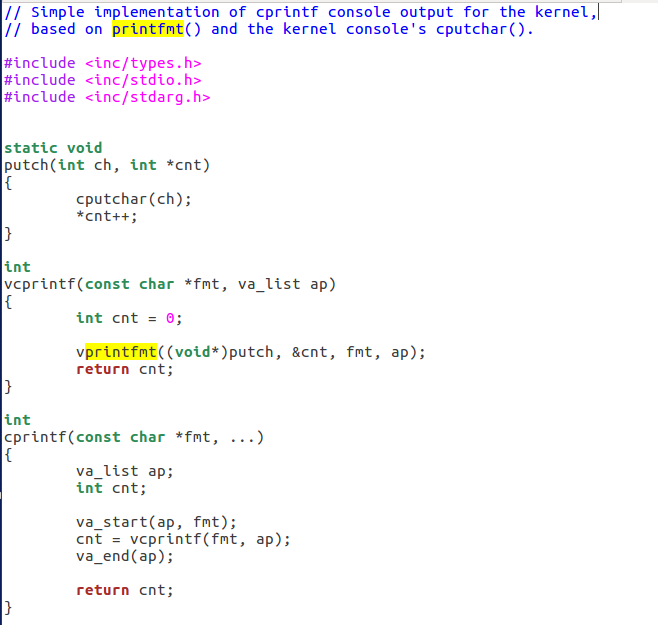
\includegraphics[width=0.8\linewidth]{figure/printf}
  \caption{printf}\label{2}
\end{figure}

In this question, we follow the case 'u' to write the code.
\begin{figure}[H]
  \centering
  % Requires \usepackage{graphicx}
  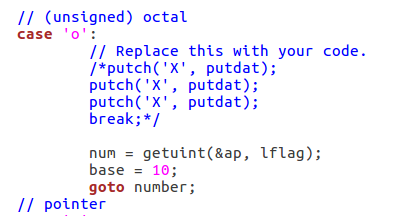
\includegraphics[width=0.8\linewidth]{figure/caseo}
  \caption{answer}\label{2}
\end{figure}

After that we modify the monitor.c file and then run qemu on the terminal to test our results.
\begin{figure}[H]
  \centering
  % Requires \usepackage{graphicx}
  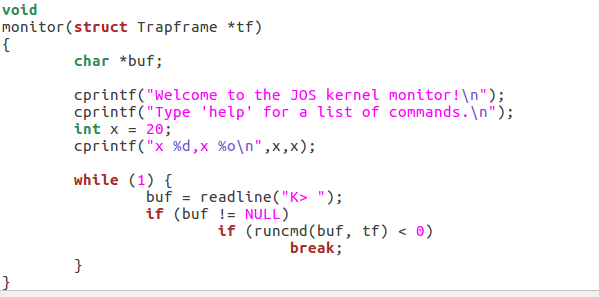
\includegraphics[width=0.8\linewidth]{figure/monitor}
  \caption{Change monitor}\label{2}
\end{figure}
\begin{figure}[H]
  \centering
  % Requires \usepackage{graphicx}
  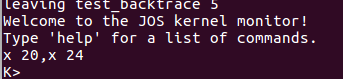
\includegraphics[width=0.8\linewidth]{figure/resultofmonitor}
  \caption{Result test}\label{2}
\end{figure}


As can be seen from the results, the 20 we defined is under \%d, and the \%o is correctly changed to octal 24

\subsubsection{Stack}
\begin{flushleft}
{\Large Exercise}

\qquad To become familiar with the C calling conventions on the x86,find the address of the test\_backtrace function in obj/kern/kernel.asm,set a breakpoint there,and examine what happens each time it gets called after the kernel starts.How many 32-bits words does each recursive nesting level of test\_backtrace push on the stack,and what are those words?\\


{\Large Answer}\\
\end{flushleft}

First, let's take a look at the source code of the test\_backtrace function in kernel.asm
\begin{figure}[H]
  \centering
  % Requires \usepackage{graphicx}
  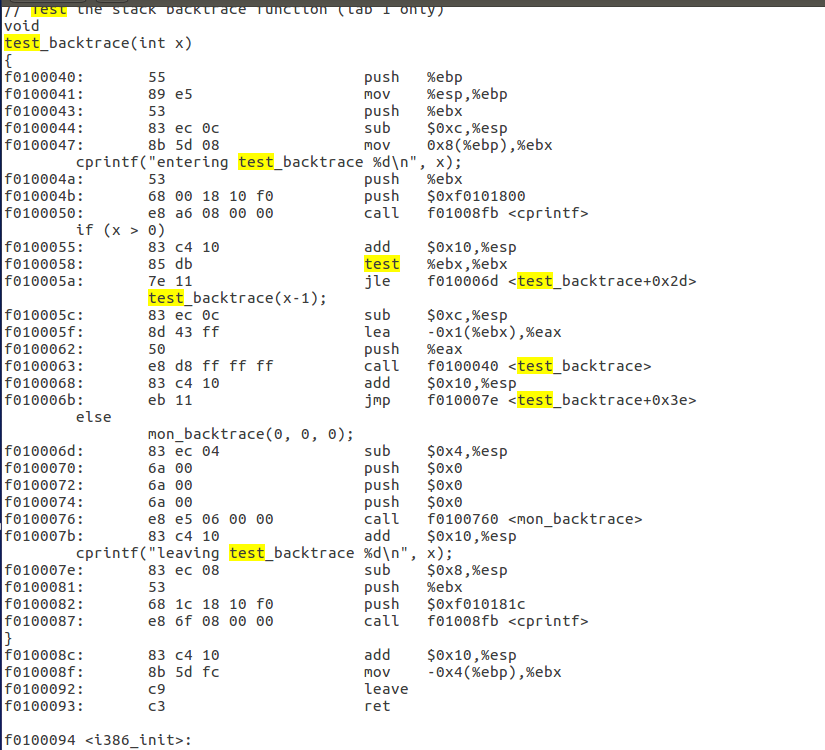
\includegraphics[width=0.8\linewidth]{figure/test_backtrace}
\end{figure}

From the code we can see the address of test\_backtrace, so we set a breakpoint here, then jump to here, as shown below:
\begin{figure}[H]
  \centering
  % Requires \usepackage{graphicx}
  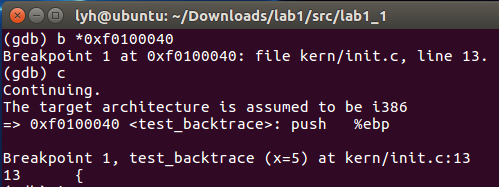
\includegraphics[width=0.8\linewidth]{figure/backtrace_set_breakpoint}
\end{figure}
Then we use the i r instruction to view the register contents and repeat the above operation
\begin{figure}[H]
  \centering
  % Requires \usepackage{graphicx}
  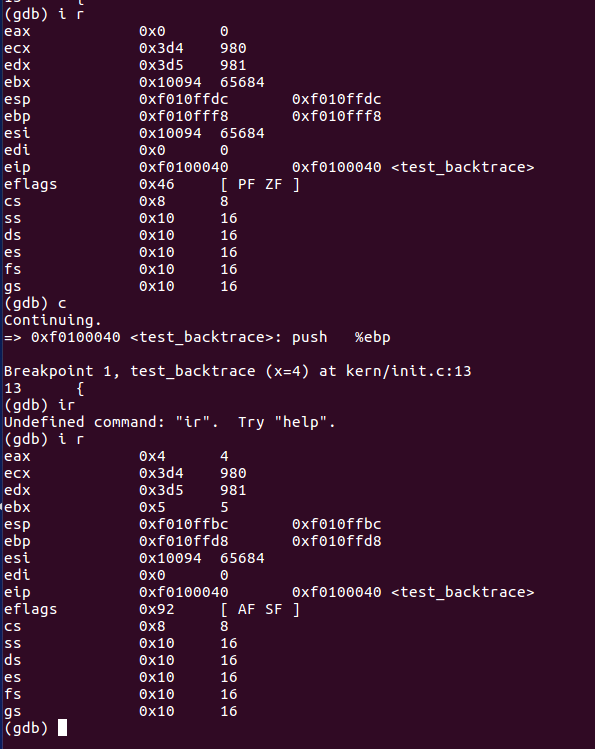
\includegraphics[width=0.8\linewidth]{figure/test_backtrace_c}
\end{figure}

By comparison, we can find that the value of ebp is reduced by 20 (hexadecimal), so we can judge every time it pushes 8 4-byte words.

According to the structure of the test\_backtrace function and the change of the stack when the function is called, each time the function is called, the ebp, the return address, the saved ebx value, and the parameters of the next call function must be pushed onto the stack. There are also 4 reserved words.

\subsubsection{Homework \Rmnum{2}}
\begin{flushleft}
{\Large Question}
\end{flushleft}

You can do mon\_backtrace() entirely in C.You'll also have to hook this new function into the kernel monitor's command list so that it can be invoked interactively by the user.The backtrace function should display a listing of function call frames in the following format:

Waring:

read\_ebp

display format

\begin{flushleft}
{\Large Answer}
\end{flushleft}



We first call the read\_ebp function to get the value of the current EBP register. We treat the entire call stack as an array, EBP[0] represents the ebp value of the previous function, and EBP [1] stores the function return address, EBP [2] What is stored later is the value of the input parameter.

\begin{table}[H]
\centering
\begin{tabular}{ |p{150pt}| }\toprule
\hline			
Ebp of the previous function  \\ \hline		
ebx \\ \hline 		
Parameter 1 \\ \hline 	
Parameter 2 \\ \hline
Parameter 3 \\ \hline
Parameter 4 \\ \hline
Parameter 5 \\ \hline
\end{tabular}
\caption{Stack structure diagram}
\end{table}

The modified mon\_backtrace function code is shown in the figure
\begin{figure}[H]
  \centering
  % Requires \usepackage{graphicx}
  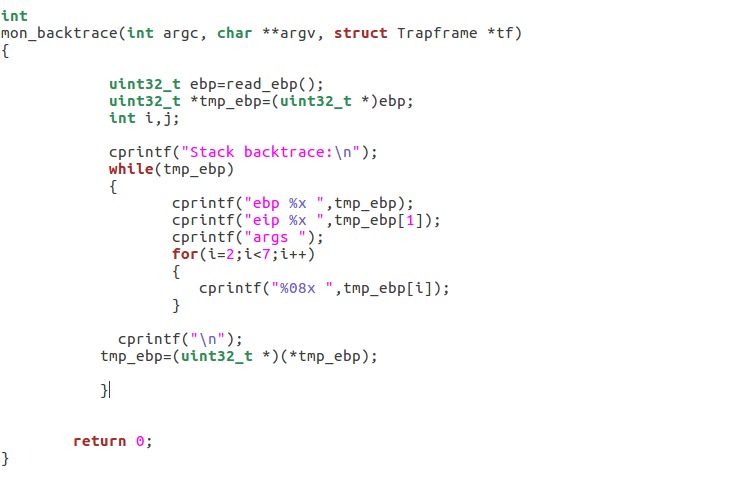
\includegraphics[width=0.8\linewidth]{figure/mon_backtrace_code}
\end{figure}

After analysis, we can know that when the function is called, the parameters are first pushed onto the stack, then the eip is pushed onto the stack, and finally the ebp is pushed onto the stack, and the new ebp points to the position of the old ebp. Therefore, the location pointed to by ebp stores the value of the previous function ebp, and the location of ebp+1 stores the value of eip. So we first print out tmp\_ebp as ebp, tmp\_ebp[1] as eip. Then we print out the values ​​of 5 parameters according to the requirements of the topic. Finally, we take the value in the memory space pointed to by ebp and repeat the above process until the first function is called.

The result of the operation is as follows
\begin{figure}[H]
  \centering
  % Requires \usepackage{graphicx}
  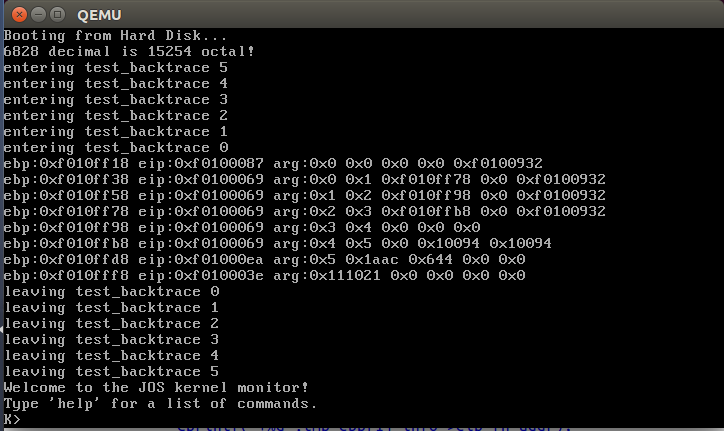
\includegraphics[width=0.8\linewidth]{figure/mon_backtrace_qemu}
\end{figure}

Add backtrace to the command list
\begin{figure}[H]
  \centering
  % Requires \usepackage{graphicx}
  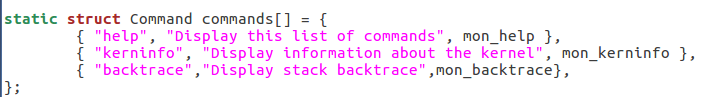
\includegraphics[width=0.8\linewidth]{figure/add_backtrace}
\end{figure}

The results are as follows:
\begin{figure}[H]
  \centering
  % Requires \usepackage{graphicx}
  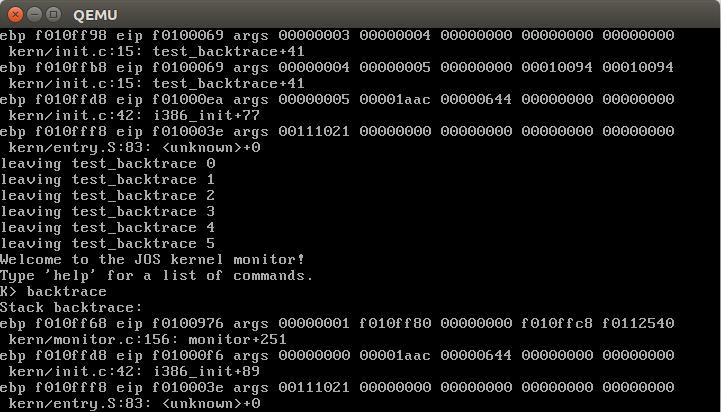
\includegraphics[width=0.8\linewidth]{figure/backtrace_result}
\end{figure}
\subsubsection{Challenge homework}
\begin{flushleft}
{\Large Question}
\end{flushleft}

Modify your stack backtrace function to display, for each eip, the function name, source file name, and line number corresponding to that eip.
In debuginfo\_eip, where do \_\_STAB\_* come from?

\begin{flushleft}
{\Large Answer}
\end{flushleft}


After reading the contents of stab.h and using the objdump -G kernel command, you can roughly know the fields of the stab table that store debugging information and their meanings, as follows

Uint32\_t n\_strx; index, can be added to stabstr to get the corresponding address of the string information.

Uint8\_t n\_type; The type of the line content, such as functions, function parameters, a line in the source file, etc.

Uint8\_t n\_other; usually empty.

Uint16\_t n\_desc; Stores the specific number of rows when type is n\_sline.

Uintptr\_t n\_value; The position of the corresponding content runtime in memory (or relative to the location where the function starts the instruction).

Collect the contents of the header file and the stab table, and analyze the meaning of each field as follows:
\begin{figure}[H]
  \centering
  % Requires \usepackage{graphicx}
  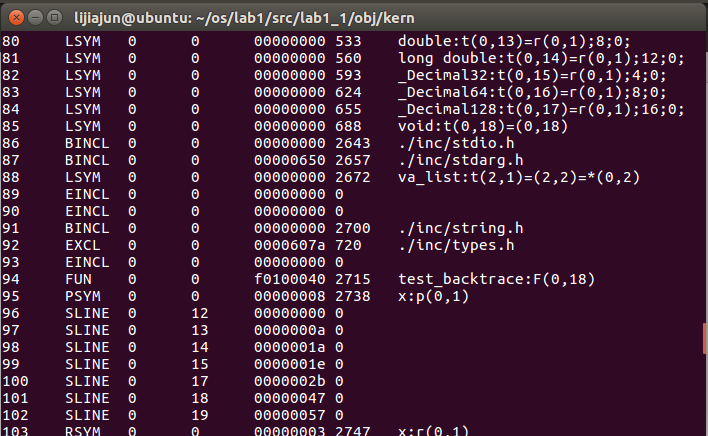
\includegraphics[width=0.8\linewidth]{figure/challenge_1}
\end{figure}

The function for finding symbol information is debuginfo\_eip(uintptr\_t addr, struct Eipdebuginfo *info)
Analysis of kdbug.h, found that the function of this function is to fill the corresponding fields of the Eipdebuginfo structure.
Analyze the debuginfo\_eip function and find that its execution logic is roughly: the structure of the eip value to be searched and the information to save the result. In the stab table, a binary search is performed on the item whose n\_type is file, and it is found that the value of the eip is in the middle of the label of the two source files (the first item in the figure). Then, the labels of the two source files are used as the left and right intervals, and the items in which the type is fun are binary searched, and the value is found between the two function labels. Finally, the eip value is subtracted from the left interval function value, and a binary search is performed to find the corresponding eip line number.
The added code is as follows:
\begin{figure}[H]
  \centering
  % Requires \usepackage{graphicx}
  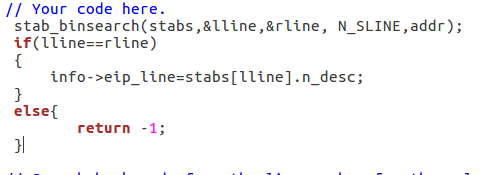
\includegraphics[width=0.8\linewidth]{figure/challenge_2}
\end{figure}


Modify the mon\_backtrace code to output the search result
\begin{figure}[H]
  \centering
  % Requires \usepackage{graphicx}
  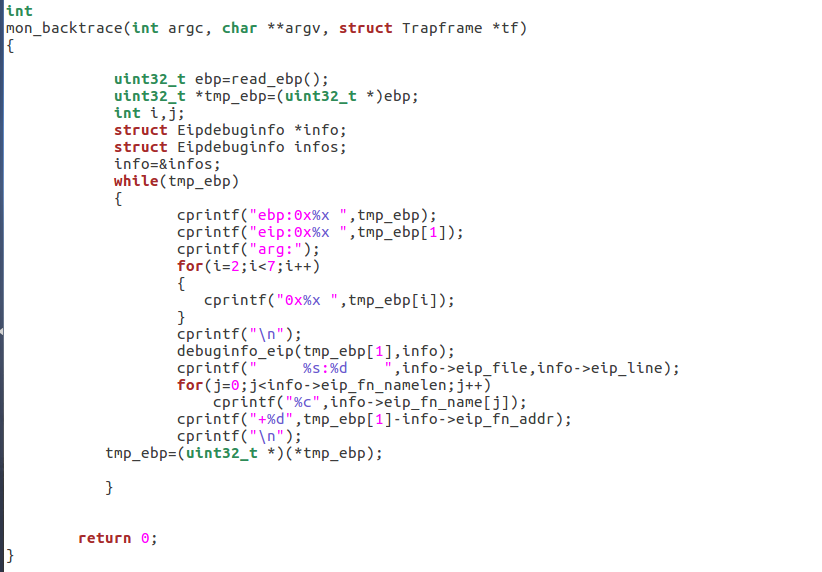
\includegraphics[width=0.8\linewidth]{figure/challenge_3}
\end{figure}

Eip\_fn\_namelen is used to exclude colon information after the function name

Tmp\_ebp[1](eip)-info->eip\_fn\_addr outputs the byte difference between the current instruction and the first instruction address of the function.
\clearpage





























